\section{Introduction}

Large models (directed labeled graphs with a inherent spanning tree) cannot be hold in computer memory. Large models need to be fragmented into smaller models. These smaller parts can be loaded and worked with. This is practical, since most application only require to handle a small part of a large model at a time. 

Large models are small enough to be stored on a single computer (non-distributed, single computer scenario). Extra large models are even to big for common hard-drives and need to be distributed over multiple computer (distributed scenario).

There are three existing fragmentation strategies:
\begin{itemize}

\item No fragmentation, the model is not fragmented. Large models are not possible.
\item Total fragmentation, each object of the model (a node with all its outgoing edges) is stored in its own fragment.
\item Manual fragmentation, the user determines which objects of a model comprise which fragments.
\end{itemize} 

There are several distinct problems with fragmentation of (extra) large models:
\begin{itemize}

\item In extreme broad models one object might be too big. Too big for memory, or too big for reasonable and efficient use. This happened for example with sensor data collected over long periods of time. On sensor (object, node) holds references (edges) to 1000s of 1000s of values.  

\item Trivial fragmentation (no oder total) might not produce optimal or even functional results. 

\item There are several parameters that influence optimal fragmentation: parsing speed, data store access speed, whether parsing or accesses different entries can be parallelized (distribute scenario). Random access (random read) vs. sequential access (scan). 

\item Fragmentation in general depends on model usage patterns. These cannot be known at model creation and might change over time.
\end{itemize}

\subsection{Terms}

Specific terms are: \emph{model}, \emph{large model}, \emph{extra large model}, \emph{fragmentation}, \emph{fragment}, \emph{no fragmentation}, \emph{total fragmentation}, \emph{manual fragmentation}, \emph{key-value data store}, \emph{entry}. Further terminology may be introduced later.

\section{Possible performance gains for loading models from local key-value data stores}

In this section, we look the possible performance gains in a non-distributed environment. This means there is only one data store that can only be accessed sequentially. 

\subsection{Optimal Fragmentation of Models}

First, we need to define a few functions that provide the performance of all operations involved in loading a model. We define the \emph{local load} function $ll$ that determines how long it takes to load a model of a given $size$  from a local data store:

$$ll:size\rightarrow t=\mathcal{O}\left(size\right)$$

The next function \emph{find entry local} $fl$ determines how long it takes to find an entry in a local key-value data store based on the number of key $\#keys$, i.e. number of entries:

$$fl:\#keys\rightarrow t=\mathcal{O}log(\#keys)$$

We will use the following parameters: The total model $size$, the average number of objects per entry $ope$, the size of the model to load $load$, and $part$ the average percentage of an entry's objects that belong to the loaded model if at least one object is part of the loaded model.

The time $t$ to load a model with this parameters is:

\begin{eqnarray*}
t&=&\frac{load}{part*ope}\left(fl(\frac{size}{ope}) + ll(ope)\right)\\
&=&\mathcal{O}\frac{load}{part*ope}\left(log(\frac{size}{ope})+ope\right)\\
\end{eqnarray*}

The two extreme examples are: (only one big entry) $ope=size$, $part=load/size$, $t=\mathcal{O}\left(size\right)$, and (one object per entry) $ope=1$, $part=1$, $t=\mathcal{O}\left(load\left(log(size)+1\right)\right)$. 

\subsubsection{Analysis}
In the optimal model distribution (one only wants to load models that exactly constitute one entry) $ope=load$ and $part=1$ the time is $t=\mathcal{O}\left(log(\frac{size}{load})+load\right)$.

\begin{figure}
  \centering
  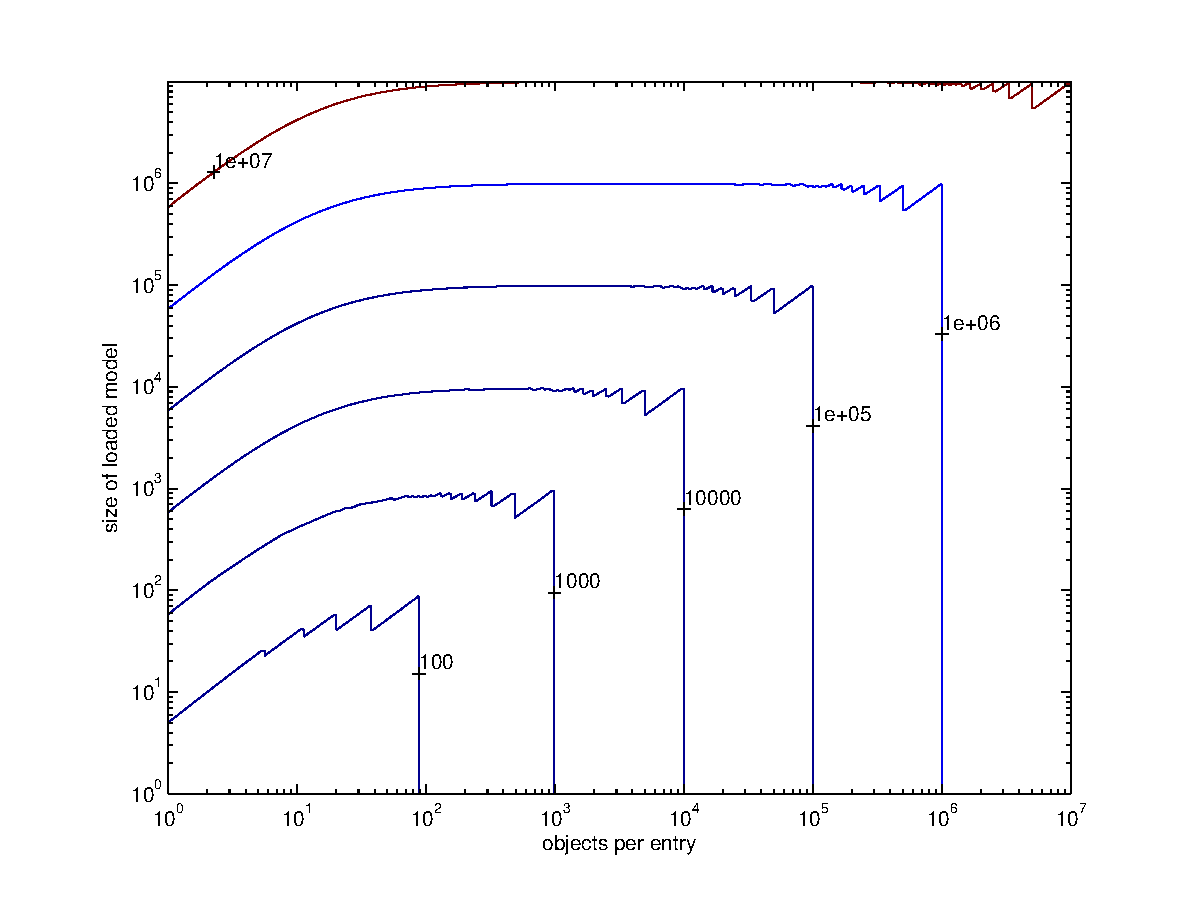
\includegraphics[width=0.65\linewidth]{figures/optimal_load_times}
  \caption{Load times}
  \label{fig:optimal_load_times}
\end{figure}

The plot in Fig.~\ref{fig:optimal_load_times} shows the relation between objects per entry, load size, and the time it takes to load. The contours show loads that take the same time. The plot does not account for any $ll=m*size+n$ and $fl=m*log(\#keys)+n$ factors ($m,n$). Depending on actual factors (see next section) the linear or logarithmic parts of the contours are more or less dominant. If parsing is relatively slow, fragmentation becomes more important (linear parts of contours are longer), if accessing the data-base becomes relatively slow, fragmentation becomes less relevant and generally large object per entry numbers are more desirable (logarithmic parts of contours are longer).

\subsubsection{Measurements}

We measured the performance of EMF parsing (depending on model size) and HBase data store access (depending on number of data store entries). The results are shown in Fig.~\ref{fig:optimal_load_times}. As expected the parsing performance is linear and the data store access behaves logarithmic. The plot in Fig.~\ref{fig:optimal_load_times_measured} is similar to Fig.~\ref{fig:optimal_load_times}, but uses $ll$ and $fl$ factors based on the measurements (actually the interpolated functions shown as lines in the plots).  

From this plot, we can see what fragmentation allows compared to no fragmentation ($ope=size$) or complete fragmentation ($ope=1$). No fragmentation always takes the full time (10s in this scenario). Of course optimal results can be obtained if ($load=ope$). This optimal result allows to load models a 1000 times bigger at the same time than total fragmentation. 

\begin{figure}[ht]
\begin{minipage}[b]{0.5\linewidth}
\centering
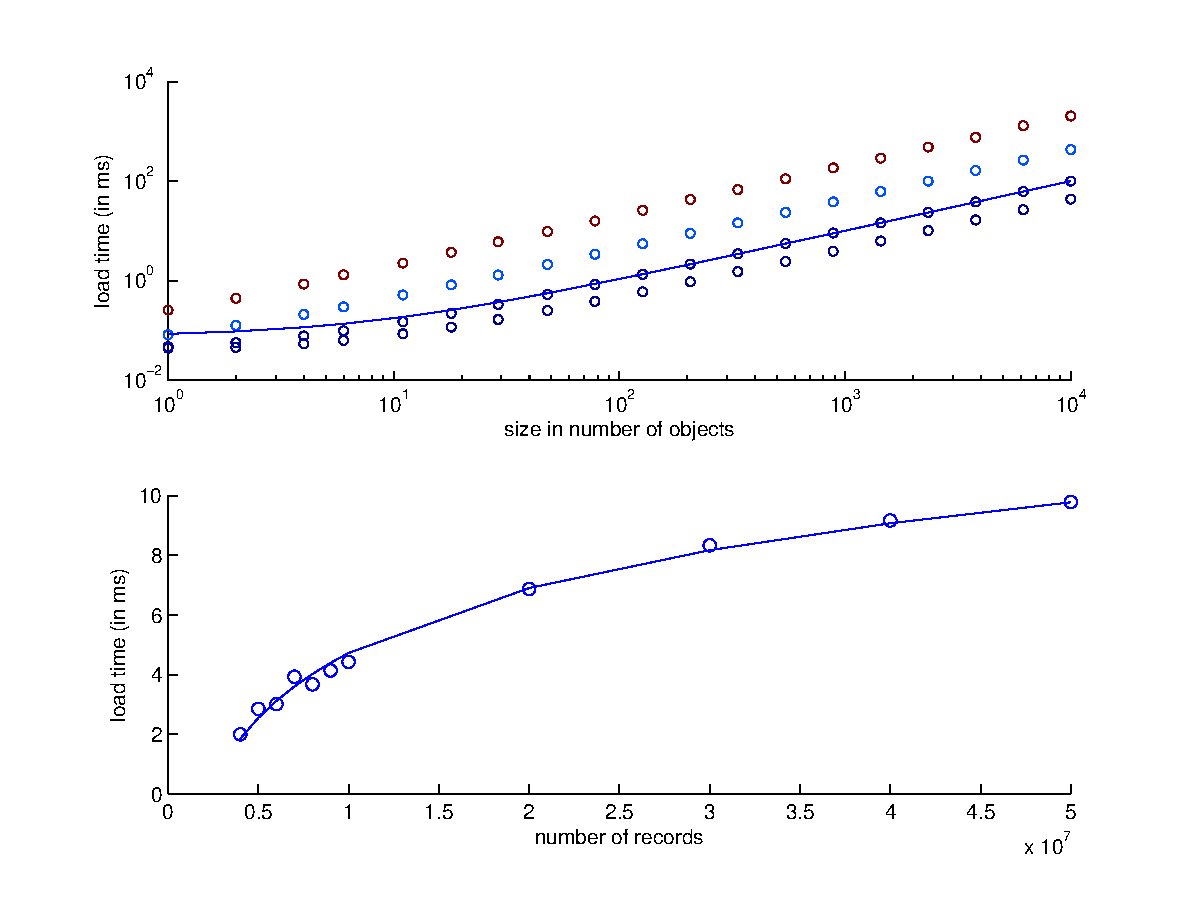
\includegraphics[width=\linewidth]{figures/emf_hbase_performance_measured}
\caption{Measure for liner parsing performance of EMF and logarithmic access performance of HBase.}
\label{fig:figures/emf_hbase_performance_measured}
\end{minipage}
\hspace{0.5cm}
\begin{minipage}[b]{0.5\linewidth}
\centering
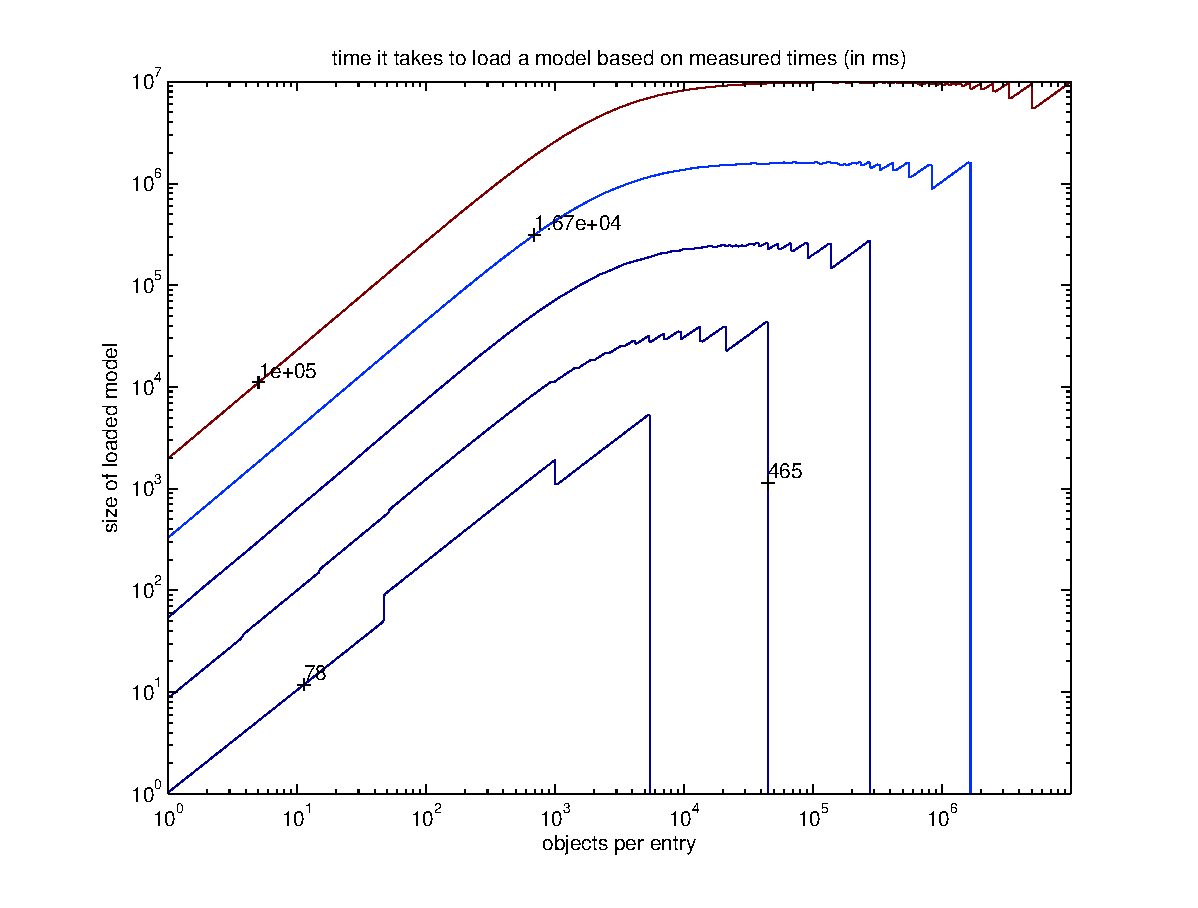
\includegraphics[width=\linewidth]{figures/optimal_load_times_measured}
\caption{Load times based on actual EMF parsing and HBase access measurements.}
\label{fig:optimal_load_times_measured}
\end{minipage}
\end{figure}

\subsection{Non Optimal Fragmentation Even Models}

\subsubsection{Analysis}

At the beginning, we will look at \emph{even} models. A model is even, if its inner structure suggest fragmentation into equal pieces. For example, an intuitive way to fragment a OO software model is to put each package into one entry. This is an uneven model, since packages have different sizes. Another example is sensor data, sensor data produced at each point in time or on each node has the same size. If one puts each sensor reading or each node into one entry, the entries will have similar size.

Previously, we were looking the gains achieved with optimal fragmentation. While optimal fragmentation is plausible in manually fragmented models for a single specific loaded model (e.g. accessing single sensor readings in ClickWatch). Optimal fragmentation is unlikely for different loaded models (even impossible for models of different size). 

In general, we can assume that the smaller $ope$ is compared to $load$, the more likely it is that much of each entry is part of the loaded model. In other words, the smaller my entries are, the more likely it is that much or all if a single entry is part of the loaded model. We will model $part$  accordingly.